\documentclass[11pt]{article}

% Keep release PDFs byte-reproducible across clean builds with the pinned TeX environment.
\ifdefined\pdfinfoomitdate\pdfinfoomitdate=1\fi
\ifdefined\pdftrailerid\pdftrailerid{}\fi
\ifdefined\pdfsuppressptexinfo\pdfsuppressptexinfo=15\fi

\usepackage[margin=1in]{geometry}
\usepackage{amsmath}
\usepackage{array}
\usepackage{authblk}
\usepackage{booktabs}
\usepackage{fancyvrb}
\usepackage{float}
\usepackage{graphicx}
\usepackage[numbers]{natbib}
\usepackage{pgfplots}
\usepackage{placeins}
\usepackage{seqsplit}
\usepackage{tikz}
\usetikzlibrary{arrows.meta,calc,patterns,positioning}
\usepgfplotslibrary{fillbetween}
\pgfplotsset{compat=1.18}
\usepackage{xcolor}
\usepackage{xurl}
\usepackage{hyperref}

\newif\ifanonymous
\ifdefined\ANONYMOUS
  \anonymoustrue
  \newcommand{\PaperPDFAuthors}{Anonymous Authors}
\else
  \anonymousfalse
  \newcommand{\PaperPDFAuthors}{Anika Datta and Anandaswarup Vadapalli}
\fi

\hypersetup{
  colorlinks=true,
  linkcolor=blue,
  citecolor=blue,
  urlcolor=blue,
  pdftitle={CrossExam: Testing a Language-Model Navigation Judge Against Exact Ground Truth},
  pdfauthor={\PaperPDFAuthors},
  pdfsubject={Testing a language-model navigation judge against exact ground truth},
  pdfkeywords={CrossExam, robot navigation, gridworld, large language model, LLM judge, exact verification, PPO}
}
% ---- begin inlined results_macros.tex ----
% Generated from frozen locked/variant aggregates and frozen pilot margins.
\newcommand{\EOneEpisodes}{1,000 groups / 5,000 trajectories}
\newcommand{\EOneSuccessAccuracy}{93.75\%}
\newcommand{\EOneSuccessAccuracyCI}{[93.06, 94.43]\%}
\newcommand{\EOneActionRegret}{0.439 steps}
\newcommand{\EOneActionRegretCI}{[0.399, 0.482]}
\newcommand{\EOneASCIIActionRegret}{0.401 steps}
\newcommand{\ImageASCIIEffect}{+1.19 pp}
\newcommand{\ImageASCIIEffectCI}{[0.36, 2.05] pp}
\newcommand{\ETwoLanguageEffect}{+7.98 pp}
\newcommand{\ETwoLanguageEffectCI}{[6.51, 9.46] pp}
\newcommand{\EThreeJudgeTransfer}{+3.77 pp}
\newcommand{\EThreeJudgeTransferCI}{[2.32, 5.98] pp}
\newcommand{\EThreeCommonSupport}{96.88\%}
\newcommand{\DecisionDamage}{0.00\%}
\newcommand{\DecisionDamageCI}{[0.00, 0.00]\%}
\newcommand{\DecisionDamageRuleThreeUpper}{0.30\%}
\newcommand{\FPEOneSuccessAccuracy}{93.79\%}
\newcommand{\FPEOneSuccessAccuracyCI}{[93.09, 94.47]\%}
\newcommand{\FPEOneActionRegret}{0.439 steps}
\newcommand{\FPEOneActionRegretCI}{[0.399, 0.482]}
\newcommand{\FPImageASCIIEffect}{+1.26 pp}
\newcommand{\FPImageASCIIEffectCI}{[0.41, 2.13] pp}
\newcommand{\FPETwoLanguageEffect}{+8.43 pp}
\newcommand{\FPETwoLanguageEffectCI}{[6.90, 9.96] pp}
\newcommand{\FPDecisionDamage}{0.10\%}
\newcommand{\FPDecisionDamageCI}{[0.00, 0.30]\%}
\newcommand{\FPEThreeJudgeTransfer}{+4.83 pp}
\newcommand{\FPEThreeJudgeTransferCI}{[3.17, 6.87] pp}
\newcommand{\CanonicalJudgeModel}{gpt\mbox{-}5.6\mbox{-}luna}
\newcommand{\CanonicalJudgeCost}{\$62.92}
\newcommand{\LockedObservations}{40,600}
\newcommand{\LockedRequests}{42,069}
\newcommand{\LockedFirstPassValid}{39,135}
\newcommand{\LockedFollowupValid}{1,128}
\newcommand{\LockedInvalid}{337}
\newcommand{\PPOValidationRange}{0.0--0.5\%}
\newcommand{\ActionOrderFlip}{34.5\%}
\newcommand{\ConsistencyDetection}{37.5\%}
\newcommand{\NoTaskUncertainty}{0.0\%}
\newcommand{\NoTaskCorrectCount}{0}
\newcommand{\NoTaskObservations}{1,000}
\newcommand{\EvidenceClaims}{109,776}
\newcommand{\CheckableEvidenceClaims}{102,985}
\newcommand{\EvidenceSupport}{48.0\%}
\newcommand{\TaskAEvidenceCheckable}{6,052}
\newcommand{\TaskAEvidenceSupported}{5,641}
\newcommand{\TaskAEvidenceSupport}{93.2\%}
\newcommand{\TaskBEvidenceCheckable}{96,933}
\newcommand{\TaskBEvidenceSupported}{43,837}
\newcommand{\TaskBEvidenceSupport}{45.2\%}
\newcommand{\EvidenceFalseStep}{12,536}
\newcommand{\EvidenceFalseCell}{20,485}
\newcommand{\EvidenceContradicted}{20,486}
\newcommand{\SuccessCalibrationECE}{0.027}
\newcommand{\ActionCalibrationECE}{0.167}
\newcommand{\FactsCalibrationECE}{0.706}
\newcommand{\SuccessCalibrationBrier}{0.029}
\newcommand{\ActionCalibrationBrier}{0.216}
\newcommand{\FactsCalibrationBrier}{0.670}
\newcommand{\SuccessCalibrationN}{29,672}
\newcommand{\ActionCalibrationN}{7,598}
\newcommand{\FactsCalibrationN}{29,672}
\newcommand{\TargetOutcomeRange}{86.4--97.8\%}
\newcommand{\AllFactsRange}{4.7--34.9\%}
\newcommand{\NormalScoringObservations}{19,436}
\newcommand{\DirectComponentsExact}{17.77\%}
\newcommand{\DirectRecomputedMAE}{0.090}
\newcommand{\RecomputedOracleMAE}{0.031}
\newcommand{\VariantRequests}{2,799}
\newcommand{\VariantCost}{\$3.58}
\newcommand{\VariantTriplets}{482}
\newcommand{\VariantIncompleteTriplets}{18}
\newcommand{\VariantPairs}{600}
\newcommand{\VariantGroups}{200}
\newcommand{\VLabelAccuracyEffect}{-0.21 pp}
\newcommand{\VLabelAccuracyEffectCI}{[-2.49, 2.07] pp}
\newcommand{\VLabelProbabilityEffect}{+0.26 pp}
\newcommand{\VLabelProbabilityEffectCI}{[-0.73, 1.27] pp}
\newcommand{\VPairwiseAccuracy}{94.58\%}
\newcommand{\VPairwiseAccuracyCI}{[93.25, 95.83]\%}
\newcommand{\VPairwiseFlip}{5.50\%}
\newcommand{\VPairwiseFlipCI}{[3.67, 7.50]\%}
\newcommand{\VPairwiseCycle}{1.00\%}
\newcommand{\VPairwiseCycleCI}{[0.00, 2.50]\%}
\newcommand{\OneWallAImageChanged}{46.3\%}
\newcommand{\OneWallAASCIIChanged}{63.8\%}
\newcommand{\OneWallAImageMoved}{67.7\%}
\newcommand{\OneWallAASCIIMoved}{76.6\%}
\newcommand{\OneWallAImageBothCorrect}{48.5\%}
\newcommand{\OneWallAASCIIBothCorrect}{57.4\%}
\newcommand{\OneWallBImageChanged}{95.4\%}
\newcommand{\OneWallBASCIIChanged}{97.2\%}
\newcommand{\OneWallBImageBothCorrect}{93.0\%}
\newcommand{\OneWallBASCIIBothCorrect}{93.9\%}
\newcommand{\OneWallAImagePairs}{499}
\newcommand{\OneWallAASCIIPairs}{500}
\newcommand{\OneWallBImagePairs}{498}
\newcommand{\OneWallBASCIIPairs}{495}
\newcommand{\MarginTargetOutcome}{5 pp}
\newcommand{\MarginActionRegret}{0.10 steps}
\newcommand{\MarginImageASCII}{3 pp}
\newcommand{\MarginLanguage}{3 pp}
\newcommand{\MarginDecisionDamage}{3 pp}
\newcommand{\MarginPPO}{5 pp}
\newcommand{\MarginOneWall}{5 pp}
\newcommand{\DamagePointThree}{0.7\%}
\newcommand{\DamagePointFive}{5.0\%}
\newcommand{\DamagePointOne}{15.9\%}
\newcommand{\EThreeVisibleObservationAccuracy}{97.82\%}
\newcommand{\EThreeVisibleMajorityAccuracy}{99.44\%}
\newcommand{\EThreeVisibleBalancedAccuracy}{61.46\%}
\newcommand{\EThreeVisibleMacroFOne}{61.53\%}
\newcommand{\EThreeNaturalObservationAccuracy}{97.66\%}
\newcommand{\EThreeNaturalMajorityAccuracy}{99.45\%}
\newcommand{\EThreeNaturalBalancedAccuracy}{51.91\%}
\newcommand{\EThreeNaturalMacroFOne}{50.30\%}
\newcommand{\MapBlindAccuracy}{79.52\%}
\newcommand{\MapBlindBalancedAccuracy}{56.16\%}
\newcommand{\MapBlindMacroFOne}{55.81\%}
\newcommand{\GreedyActionRegret}{0.489 steps}
\newcommand{\UniformActionRegret}{0.989 steps}
\newcommand{\UniqueStarts}{631}
\newcommand{\UniqueTargets}{628}
\newcommand{\WallDensityRange}{15.5--56.2\%}
\newcommand{\MazeFamilyImageRegretRange}{0.18--0.91 steps}
\newcommand{\AblationCases}{500}
\newcommand{\AblationObservations}{2,000}
\newcommand{\AblationRequests}{2,050}
\newcommand{\AblationCost}{\$3.02}
\newcommand{\AblationQuadruplets}{495}
\newcommand{\AblationActionsTarget}{62.9\%}
\newcommand{\AblationActionsFacts}{24.4\%}
\newcommand{\AblationIntermediateTarget}{78.6\%}
\newcommand{\AblationFinalTarget}{93.0\%}
\newcommand{\AblationFinalFacts}{36.1\%}
\newcommand{\AblationFullTarget}{94.6\%}
\newcommand{\AblationFullTargetCI}{[92.6, 96.4]\%}
\newcommand{\AblationFullFacts}{34.5\%}
\newcommand{\AblationFullFactsCI}{[30.5, 38.8]\%}
\newcommand{\AblationIntermediateNoFinalTarget}{+15.7 pp}
\newcommand{\AblationIntermediateNoFinalTargetCI}{[10.8, 20.5] pp}
\newcommand{\AblationIntermediateWithFinalTarget}{+1.6 pp}
\newcommand{\AblationIntermediateWithFinalTargetCI}{[-1.0, 4.2] pp}
\newcommand{\AblationFinalNoIntermediateTarget}{+30.0 pp}
\newcommand{\AblationFinalNoIntermediateTargetCI}{[25.6, 34.4] pp}
\newcommand{\AblationFinalWithIntermediateTarget}{+16.1 pp}
\newcommand{\AblationFinalWithIntermediateTargetCI}{[12.4, 19.9] pp}
\newcommand{\AblationIntermediateWithFinalFacts}{-1.6 pp}
\newcommand{\AblationIntermediateWithFinalFactsCI}{[-5.6, 2.6] pp}
\newcommand{\AblationTargetInteraction}{-13.9 pp}
\newcommand{\AblationTargetInteractionCI}{[-19.6, -8.5] pp}
\newcommand{\AblationFactsInteraction}{-6.7 pp}
\newcommand{\AblationFactsInteractionCI}{[-12.3, -1.0] pp}
\newcommand{\AblationFirstPassTargetInteraction}{-13.5 pp}
\newcommand{\AblationFirstPassFactsInteraction}{-7.0 pp}
\newcommand{\AblationFreshLockedAgreement}{92.8\%}
\newcommand{\AblationFreshLockedFieldsAgreement}{25.8\%}
%% ---- end inlined results_macros.tex ----
% ---- begin inlined phase_k_results_macros.tex ----
% Generated from results/phase-k-v1/aggregate; do not edit by hand.
\newcommand{\PhaseKLowEvidence}{57.4\%}
\newcommand{\PhaseKLowEvidenceCI}{[54.5, 60.4]\%}
\newcommand{\PhaseKLowFacts}{35.8\%}
\newcommand{\PhaseKLowFactsCI}{[30.3, 41.2]\%}
\newcommand{\PhaseKLowRegret}{0.454}
\newcommand{\PhaseKLowRegretCI}{[0.381, 0.531]}
\newcommand{\PhaseKLowOutcome}{93.3\%}
\newcommand{\PhaseKLowOutcomeCI}{[90.5, 95.8]\%}
\newcommand{\PhaseKLowECE}{0.580}
\newcommand{\PhaseKLowECECI}{[0.528, 0.630]}
\newcommand{\PhaseKLowAAFlip}{35.0\%}
\newcommand{\PhaseKLowAAFlipCI}{[30.2, 40.0]\%}
\newcommand{\PhaseKMediumEvidence}{65.2\%}
\newcommand{\PhaseKMediumEvidenceCI}{[62.2, 68.3]\%}
\newcommand{\PhaseKMediumFacts}{54.4\%}
\newcommand{\PhaseKMediumFactsCI}{[48.7, 60.1]\%}
\newcommand{\PhaseKMediumRegret}{0.358}
\newcommand{\PhaseKMediumRegretCI}{[0.287, 0.432]}
\newcommand{\PhaseKMediumOutcome}{97.7\%}
\newcommand{\PhaseKMediumOutcomeCI}{[96.2, 99.0]\%}
\newcommand{\PhaseKMediumECE}{0.419}
\newcommand{\PhaseKMediumECECI}{[0.366, 0.473]}
\newcommand{\PhaseKMediumAAFlip}{37.3\%}
\newcommand{\PhaseKMediumAAFlipCI}{[32.2, 42.2]\%}
\newcommand{\PhaseKHighEvidence}{68.4\%}
\newcommand{\PhaseKHighEvidenceCI}{[64.6, 72.3]\%}
\newcommand{\PhaseKHighFacts}{79.9\%}
\newcommand{\PhaseKHighFactsCI}{[75.4, 84.1]\%}
\newcommand{\PhaseKHighRegret}{0.305}
\newcommand{\PhaseKHighRegretCI}{[0.234, 0.378]}
\newcommand{\PhaseKHighOutcome}{97.6\%}
\newcommand{\PhaseKHighOutcomeCI}{[95.8, 99.0]\%}
\newcommand{\PhaseKHighECE}{0.172}
\newcommand{\PhaseKHighECECI}{[0.134, 0.210]}
\newcommand{\PhaseKHighAAFlip}{32.0\%}
\newcommand{\PhaseKHighAAFlipCI}{[27.2, 36.8]\%}
\newcommand{\PhaseKLowPrimaryAAFlip}{36.5\%}
\newcommand{\PhaseKLowPrimaryAAFlipCI}{[29.5, 43.0]\%}
\newcommand{\PhaseKHighTaskBValid}{88.5\%}
\newcommand{\PhaseKHighTaskBInvalid}{69}
\newcommand{\PhaseKHighFactsMissingLower}{72.3\%}
\newcommand{\PhaseKHighFactsMissingUpper}{83.8\%}
\newcommand{\PhaseKHighOutcomeMissingLower}{86.2\%}
\newcommand{\PhaseKHighOutcomeMissingUpper}{97.7\%}
\newcommand{\PhaseKRequests}{4,400}
\newcommand{\PhaseKValid}{4,307}
\newcommand{\PhaseKCost}{\$9.17}
\newcommand{\PhaseKHighLowCostMultiple}{4.38x}
%% ---- end inlined phase_k_results_macros.tex ----
% ---- begin inlined phase_l_results_macros.tex ----
% Generated from results/phase-l-v1/aggregate; do not edit by hand.
\newcommand{\PhaseLRequests}{1,400}
\newcommand{\PhaseLValid}{1,398}
\newcommand{\PhaseLCost}{\$0.98}
\newcommand{\PhaseLAAFlip}{32.0\%}
\newcommand{\PhaseLAAFlipCI}{[25.5, 38.5]\%}
\newcommand{\PhaseLChangedFlip}{37.7\%}
\newcommand{\PhaseLChangedFlipCI}{[33.0, 42.5]\%}
\newcommand{\PhaseLOrderExcess}{+5.7 pp}
\newcommand{\PhaseLOrderExcessCI}{[-0.2, +11.7] pp}
\newcommand{\PhaseLMovementExcess}{+0.014}
\newcommand{\PhaseLMovementExcessCI}{[-0.028, +0.055]}
\newcommand{\PhaseLLowNoTaskCorrect}{0}
\newcommand{\PhaseLLowNoTaskValid}{199}
\newcommand{\PhaseLLowNoTaskRate}{0.0\%}
\newcommand{\PhaseLLowNoTaskRateCI}{[0.0, 0.0]\%}
\newcommand{\PhaseLLowNoTaskRuleThreeUpper}{1.5\%}
\newcommand{\PhaseLHighNoTaskCorrect}{3}
\newcommand{\PhaseLHighNoTaskValid}{199}
\newcommand{\PhaseLHighNoTaskRate}{1.5\%}
\newcommand{\PhaseLHighNoTaskRateCI}{[0.0, 3.5]\%}
\newcommand{\PhaseLHighNoTaskFailure}{98.5\%}
\newcommand{\PhaseLNoTaskPairs}{198}
\newcommand{\PhaseLNoTaskDifference}{+1.5 pp}
\newcommand{\PhaseLNoTaskDifferenceCI}{[+0.0, +3.5] pp}
%% ---- end inlined phase_l_results_macros.tex ----
% ---- begin inlined budget_response_macros.tex ----
% Generated from results/budget-response-v1; do not edit by hand.
\newcommand{\BudgetFactsGain}{+42.6 pp}
\newcommand{\BudgetEvidenceGain}{+11.0 pp}
\newcommand{\BudgetStabilityGain}{+3.0 pp}
\newcommand{\BudgetContractGain}{+1.5 pp}
\newcommand{\LockedInsufficientCount}{1,000}
\newcommand{\LockedTaskInvalidCount}{0}
\newcommand{\PhaseLLowInsufficientCount}{199}
\newcommand{\PhaseLHighInsufficientCount}{199}
\newcommand{\PhaseLHighTaskInvalidCount}{3}
%% ---- end inlined budget_response_macros.tex ----
% ---- begin inlined convergence_results_macros.tex ----
% Generated from results/convergence-v1; do not edit by hand.
\newcommand{\ConvergenceGroups}{200}
\newcommand{\ConvergenceCalls}{4,400}
\newcommand{\ConvergenceStatus}{complete post-hoc offline recount}
\newcommand{\ConvergenceOneLowTaskACorrect}{77.3\%}
\newcommand{\ConvergenceOneLowTaskAUnresolved}{0.0\%}
\newcommand{\ConvergenceOneLowTargetCorrect}{91.5\%}
\newcommand{\ConvergenceOneLowTargetUnresolved}{1.9\%}
\newcommand{\ConvergenceOneLowFactsCorrect}{35.8\%}
\newcommand{\ConvergenceOneLowFactsWrong}{62.3\%}
\newcommand{\ConvergenceOneLowFactsUnresolved}{1.9\%}
\newcommand{\ConvergenceFiveLowFactsWrong}{3.5\%}
\newcommand{\ConvergenceFiveLowTaskACorrect}{77.0\%}
\newcommand{\ConvergenceOneHighTaskACorrect}{81.8\%}
\newcommand{\ConvergenceFiveLowTaskAUnresolved}{6.0\%}
\newcommand{\ConvergenceOneHighTaskAUnresolved}{0.2\%}
\newcommand{\ConvergenceFiveLowTargetCorrect}{95.0\%}
\newcommand{\ConvergenceOneHighTargetCorrect}{86.2\%}
\newcommand{\ConvergenceFiveLowTargetUnresolved}{1.0\%}
\newcommand{\ConvergenceOneHighTargetUnresolved}{11.5\%}
\newcommand{\ConvergenceFiveLowFactsCorrect}{38.5\%}
\newcommand{\ConvergenceOneHighFactsCorrect}{72.3\%}
\newcommand{\ConvergenceFiveLowFactsUnresolved}{58.0\%}
\newcommand{\ConvergenceOneHighFactsUnresolved}{11.5\%}
\newcommand{\ConvergenceOneHighTargetValidOnly}{97.6\%}
\newcommand{\ConvergenceOneHighFactsValidOnly}{79.9\%}
\newcommand{\ConvergenceHighTaskBValidRate}{88.5\%}
\newcommand{\ConvergenceFiveLowTaskACost}{\$0.003353}
\newcommand{\ConvergenceOneHighTaskACost}{\$0.002766}
\newcommand{\ConvergenceTaskACostMultiple}{1.21}
\newcommand{\ConvergenceFiveLowTaskBCost}{\$0.006320}
\newcommand{\ConvergenceOneHighTaskBCost}{\$0.005712}
\newcommand{\ConvergenceTaskBCostMultiple}{1.11}
\newcommand{\ConvergenceBFSMedian}{818}
\newcommand{\ConvergenceBFSIQR}{740--847}
\newcommand{\ConvergenceReplayMedian}{39.5}
\newcommand{\ConvergenceReplayIQR}{26.75--64}
\newcommand{\ConvergenceShortestMedian}{28}
\newcommand{\ConvergenceHistoricalCost}{\$79.66}
%% ---- end inlined convergence_results_macros.tex ----
% ---- begin inlined progressive_input_results_macros.tex ----
% Generated from results/progressive-input-v1/analysis.json; do not edit.
% Base result manifest SHA-256: 95631f43febc3cbb1a109dedbb938d1f2bf202fb4fef318cab39a90d48e3445f
\newcommand{\ProgressiveCases}{200}
\newcommand{\ProgressiveStages}{9}
\newcommand{\ProgressiveCalls}{5,400}
\newcommand{\ProgressiveValidCalls}{5,397}
\newcommand{\ProgressiveIncompleteCalls}{2}
\newcommand{\ProgressiveInvalidCalls}{1}
\newcommand{\ProgressiveBaselineAccuracy}{22.7\%}
\newcommand{\ProgressiveFullAccuracy}{35.7\%}
\newcommand{\ProgressiveAccuracyGain}{+13.0 pp}
\newcommand{\ProgressiveAccuracyGainCI}{[+7.0 pp, +19.2 pp]}
\newcommand{\ProgressiveBaselineBrier}{0.894}
\newcommand{\ProgressiveFullBrier}{0.885}
\newcommand{\ProgressiveBrierChange}{-0.0085}
\newcommand{\ProgressiveBrierChangeCI}{[-0.0602, +0.0429]}
\newcommand{\ProgressivePeakAccuracy}{36.0\%}
\newcommand{\ProgressivePeakStage}{6/8}
\newcommand{\ProgressiveAccuracyDecreases}{178}
\newcommand{\ProgressiveProbabilityDecreases}{788}
\newcommand{\ProgressiveBrierIncreases}{805}
\newcommand{\ProgressiveTransitions}{1,600}
\newcommand{\ProgressiveNeverHighCorrect}{187}
\newcommand{\ProgressiveEverHighCorrect}{13}
\newcommand{\ProgressiveLaterReversals}{12}
\newcommand{\ProgressiveFullSufficient}{3.5\%}
\newcommand{\ProgressiveFullSelectiveAccuracy}{0.0\%}
\newcommand{\ProgressiveSufficientCalls}{21}
\newcommand{\ProgressiveSufficientCases}{16}
\newcommand{\ProgressiveConfidenceThreshold}{0.8}
\newcommand{\ProgressiveBalancedBaseline}{25.0\%}
\newcommand{\ProgressiveBaselineSufficient}{2.7\%}
\newcommand{\ProgressivePeakSufficient}{8.7\%}
\newcommand{\ProgressivePeakSufficientStage}{7/8}
\newcommand{\ProgressiveOutcomeCases}{50}
\newcommand{\ProgressiveBaselineECE}{0.256}
\newcommand{\ProgressiveFullECE}{0.221}
\newcommand{\ProgressiveCorrectFull}{96.7\%}
\newcommand{\ProgressiveNeitherFull}{43.3\%}
\newcommand{\ProgressiveWrongObjectFull}{2.7\%}
\newcommand{\ProgressiveWrongRelationFull}{0.0\%}
\newcommand{\ProgressiveCorrectGain}{+69.3 pp}
\newcommand{\ProgressiveNeitherGain}{-19.3 pp}
%% ---- end inlined progressive_input_results_macros.tex ----
\pgfplotstableread[col sep=comma]{generated/figures/phase_k_effort.csv}\phasekeffortdata
\pgfplotstableread[col sep=comma]{generated/figures/progressive_input_reveal.csv}\progressiverevealdata
\pgfplotstablegetelem{0}{locked_reference}\of\phasekeffortdata
\edef\PhaseKRefEvidence{\pgfplotsretval}
\pgfplotstablegetelem{3}{locked_reference}\of\phasekeffortdata
\edef\PhaseKRefFacts{\pgfplotsretval}
\pgfplotstablegetelem{6}{locked_reference}\of\phasekeffortdata
\edef\PhaseKRefRegret{\pgfplotsretval}
\pgfplotstablegetelem{9}{locked_reference}\of\phasekeffortdata
\edef\PhaseKRefOutcome{\pgfplotsretval}
\pgfplotstablegetelem{12}{locked_reference}\of\phasekeffortdata
\edef\PhaseKRefECE{\pgfplotsretval}
\pgfplotstablegetelem{15}{locked_reference}\of\phasekeffortdata
\edef\PhaseKRefFlip{\pgfplotsretval}
\setlength{\emergencystretch}{2em}
\definecolor{figureblue}{RGB}{37,99,235}
\definecolor{figuregold}{RGB}{217,119,6}
\definecolor{figureneutral}{RGB}{71,85,105}
\tikzset{
  flowbox/.style={draw, rounded corners, align=center, fill=blue!5,
    minimum height=9mm, text width=2.35cm, font=\small},
  exactbox/.style={flowbox, fill=green!8},
  flowarrow/.style={-{Latex[length=2mm]}, thick}
}

\title{CrossExam: Testing a Language-Model Navigation Judge Against Exact Ground Truth}
\ifanonymous
  \author{Anonymous Authors}
  \affil{Affiliations withheld for review}
\else
  \author[1]{Anika Datta}
  \author[2]{Anandaswarup Vadapalli}
  \affil[1]{Independent Researcher}
  \affil[2]{Research Spark Hub Inc.}
\fi
\date{August 2026}

\begin{document}
\maketitle

\begin{abstract}
Language models are increasingly used to evaluate agent behaviour, but agreement on a final outcome may conceal errors in the facts supporting that judgment. This study examines this problem in a $32\times32$ navigation environment where exact simulation and breadth-first search provide ground truth. We evaluate \CanonicalJudgeModel{} on 1,000 map--task groups, comparing action recommendations, trajectory facts, confidence, and structured evidence across image and text inputs. At low reasoning effort, target-outcome accuracy was \EOneSuccessAccuracy{} (95\% CI \EOneSuccessAccuracyCI), whereas only \TaskBEvidenceSupport{} of checkable trajectory-evidence claims were supported. Expected first-action regret was \EOneActionRegret. Follow-up experiments examined visual information, reasoning effort, repeated judgments, and progressively revealed trajectories. Increasing reasoning effort together with the output limit improved complete-fact accuracy from \PhaseKLowFacts{} to \PhaseKHighFacts{} among valid responses, although \PhaseKHighTaskBInvalid{} of 600 high-effort trajectory judgments failed to complete within the token limit. Repeated low-effort judgments improved outcome classification but provided little improvement in complete-fact recovery. Revealing all recorded actions increased accuracy on a separate, outcome-balanced sample from \ProgressiveBaselineAccuracy{} to \ProgressiveFullAccuracy{}, with gains concentrated in successful trajectories. These findings show that outcome accuracy, factual correctness, and evidence quality require separate evaluation when language models are used as judges.
\end{abstract}

\section{Introduction}
\label{sec:intro}
Reinforcement learning depends on a reward function that represents the intended task~\citep{sutton2018rl}. When this specification is incomplete, an agent may obtain a high reward without producing the desired behaviour~\citep{amodei2016concrete}. Natural-language instructions make reward specification particularly challenging because the system must interpret the instruction and determine whether an observed trajectory satisfies it.

Large language models (LLMs) offer one approach to this problem. They can generate executable reward functions or directly judge an agent's behaviour from a task description and observations~\citep{ma2024eureka,xie2024text2reward,ma2024gvl}. Direct evaluation is flexible, but it introduces a second source of uncertainty: the evaluator may misinterpret the task, misread the environment, or report facts that are inconsistent with the trajectory. A correct final label does not establish that the underlying evaluation is reliable.

This paper investigates these errors in a controlled navigation task. We use a fully specified gridworld in which breadth-first search and exact trajectory replay determine the correct answer to every evaluated question. This allows us to assess a language-model judge without relying on another learned evaluator or subjective annotations. The environment serves as a diagnostic setting for learned judgment; exact software remains the reference for task correctness.

We address three questions. First, how closely does final-outcome accuracy reflect the quality of action recommendations, trajectory facts, and supporting evidence? Second, how do input representation, visual state information, and inference budget affect these measures? Third, do repeated judgments and additional trajectory information improve the decisions made from the model's outputs?

We evaluate one judge on 1,000 map--task groups, each containing five rule-generated trajectories, and on a separate set of trajectories from policies trained with proximal policy optimization (PPO). Paired experiments compare image and ASCII maps, natural and structured instructions, and minimal changes to the environment. Follow-up studies examine visual frames, reasoning effort, response variability, and progressive trajectory reveal. Throughout the analysis, we distinguish the main study from exploratory follow-ups and report limitations that affect the interpretation of each comparison.

The remainder of the paper reviews previous work in Section~\ref{sec:related}, describes the novelty and contributions in Sections~\ref{sec:novelty} and~\ref{sec:contribution}, and presents the experimental setup in Section~\ref{sec:setup}. Section~\ref{sec:results} reports the results and their implications. Section~\ref{sec:conclusion} concludes the paper.

\section{Previous Work}
\label{sec:related}
\subsection{Reward specification and language-conditioned navigation}
Hand-designed rewards provide precise and inexpensive feedback when the task can be expressed in terms of simulator state. Potential-based reward shaping formalizes conditions under which additional feedback preserves the optimal policy~\citep{ng1999shaping}. However, interpreting new language instructions often requires additional rules. BabyAI and MiniGrid provide compact environments for studying grounded language and navigation under controlled conditions~\citep{chevalierboisvert2019babyai,chevalierboisvert2023minigrid}. Our environment follows this general approach while retaining complete observability and exact trajectory labels.

LLM-based reward design can reduce the need for manual specification. Eureka and Text2Reward generate reward code from task descriptions and feedback~\citep{ma2024eureka,xie2024text2reward}. Once selected, this code computes rewards without requiring the LLM to judge each trajectory. Direct visual evaluation takes a different approach: Generative Value Learning estimates task progress from image sequences, while RoboReward studies vision-language reward models using robot trajectories~\citep{ma2024gvl,lee2026roboreward}. Our study examines the correctness of direct judgments at the level of individual facts and evidence claims.

\subsection{Evaluating language-model judges}
LLM judges can agree with human preferences while remaining sensitive to presentation order and other properties unrelated to answer quality~\citep{zheng2023judging}. JudgeBench and RewardBench~2 evaluate judges and reward models using difficult comparisons with independently established answers~\citep{tan2025judgebench,malik2026rewardbench2}. Work on self-verification also shows why external correctness checks are valuable for reasoning and planning tasks~\citep{stechly2024selfverification}.

Spatial benchmarks further distinguish map interpretation from planning. Lost in Aggregation compares spatial navigation across representations and scales, while From Pixels to BFS separates visual extraction from subsequent search~\citep{jiang2026lost,rodriguez2026pixels}. Judge-based selection has also been examined in table recognition, where deterministic evaluation can reveal limitations of model-assigned scores~\citep{kim2026judge}. These studies motivate evaluating both the content of a judgment and the consequence of using it.

\subsection{Inference budget, repetition, and uncertainty}
Additional inference computation can be allocated to a longer generation or to multiple sampled responses. These strategies need not improve the same aspects of performance~\citep{hariri2026testtime}. Self-consistency aggregates answers from multiple reasoning paths~\citep{wang2023selfconsistency}; repeated sampling studies show that producing a correct candidate and selecting it reliably are distinct problems~\citep{brown2024monkeys}. We therefore evaluate single-response effort and repeated-response aggregation separately.

Confidence and abstention introduce a related distinction. Selective classification measures the trade-off between coverage and error when a system can withhold a prediction~\citep{geifman2017selective}, while language-model self-knowledge studies examine whether models can estimate their own correctness~\citep{kadavath2022know}. We compare confidence with exact labels and also test whether the judge recognizes a missing task specification.

\section{Novelty}
\label{sec:novelty}
CrossExam combines outcome evaluation, action evaluation, factual verification, and evidence checking within the same navigation environment. The exact simulator makes it possible to distinguish a correct outcome label from an accurate account of how that outcome occurred. Paired changes to maps and inputs then test which information affects the judgment.

The contribution lies in this combined evaluation rather than in introducing objective judge benchmarks or image--text comparisons individually. The study also connects response quality to best-of-five trajectory selection and compares two ways of increasing inference computation. A separate progressive-reveal experiment tests how predictions change as more of the same trajectory becomes visible. These comparisons provide complementary evidence about the reliability of the evaluated judge, without assuming that one accuracy measure represents all of its capabilities.

\section{Contribution}
\label{sec:contribution}
This paper makes three contributions:
\begin{enumerate}
  \item An exact-oracle evaluation of action quality, eight trajectory facts, confidence, and structured evidence on 1,000 map--task groups.
  \item Controlled comparisons of map representation, instruction form, visual frames, and inference budget, together with matched tests of presentation order and ordinary response variability.
  \item An analysis of how judgment errors affect trajectory selection, repeated-response aggregation, and outcome prediction as trajectory information is progressively revealed.
\end{enumerate}

\section{Experimental Setup}
\label{sec:setup}
\subsection{Navigation environment and trajectories}
The environment is a fully observable $32\times32$ grid. Coordinates are given as row and column, with $(0,0)$ at the upper-left. The robot can move up, right, down, or left. A move into a wall, an object, or the grid boundary leaves the robot in place and counts as a collision. Episodes end when the task is completed or after 64 actions.

Each map contains three labelled, non-traversable objects: a chair, a sofa, and a cube. Tasks specify an object and one of five relations: north, south, west, east, or at. The coordinate frame is stated in the input. Five seeded generators produce gates, switchbacks, broken rooms, corridors, and connected random blocks. Unreachable tasks and ambiguous targets that also satisfy a distractor task are rejected. The primary tasks begin 16--48 shortest-path steps from the goal. The main sample contains \UniqueStarts{} distinct starting cells, \UniqueTargets{} target cells, and wall densities spanning \WallDensityRange.

Each of the 1,000 map--task groups contains five rule-policy trajectories. The first four use exact or near-exact navigation and three levels of continuous action-replacement noise. The fifth is a constructed case drawn from six types: stopping one cell short, reaching the wrong object, satisfying the wrong relation, making one collision before succeeding, completing a loop before succeeding, or timing out beside the target. Construction rules isolate the intended error; for example, wrong-object and wrong-relation paths are collision-free, and the timeout path never enters the goal. This produces 5,000 trajectories while retaining groups as the unit for statistical analysis and candidate selection.

Development, pilot, training, stability, and main-study map seeds are disjoint. Maps, trajectories, input representations, and oracle labels were fixed before the corresponding evaluation calls. Figure~\ref{fig:environment} illustrates the environment and a one-wall intervention.

\begin{figure}[t]
\centering
\begin{minipage}[t]{0.29\linewidth}
\centering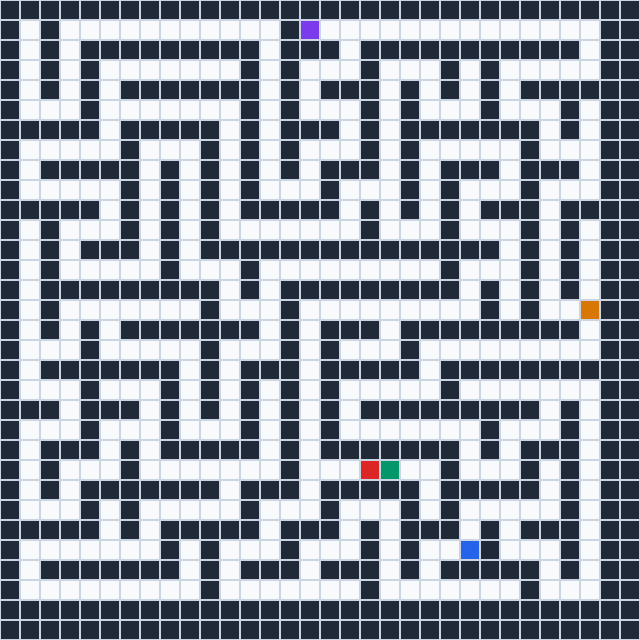
\includegraphics[width=\linewidth]{generated/figures/maze_corridors.png}\\
\small (a) Corridor layout
\end{minipage}\hfill
\begin{minipage}[t]{0.29\linewidth}
\centering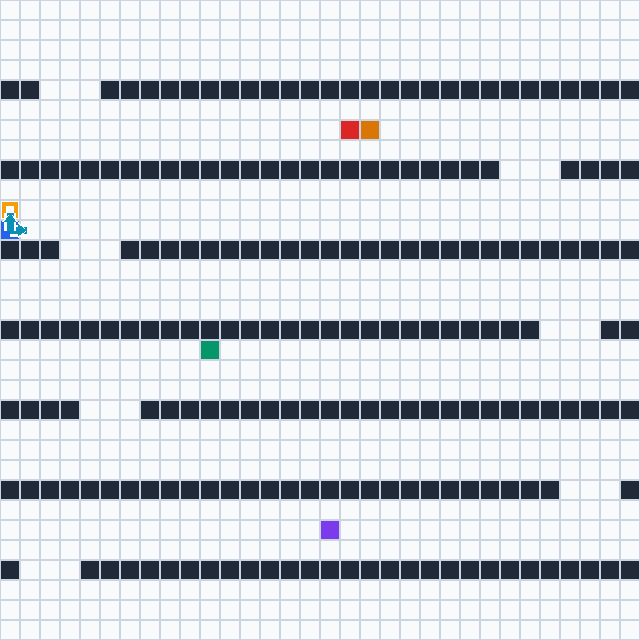
\includegraphics[width=\linewidth]{generated/figures/locked_one_wall_original.png}\\
\small (b) Original map
\end{minipage}\hfill
\begin{minipage}[t]{0.29\linewidth}
\centering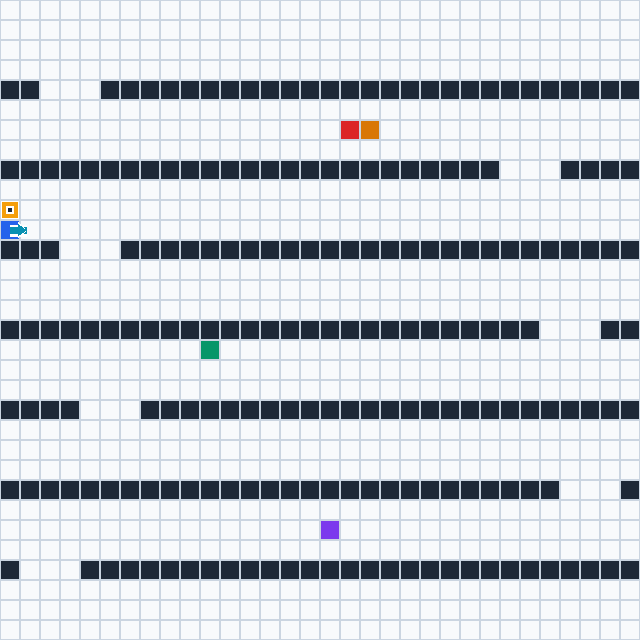
\includegraphics[width=\linewidth]{generated/figures/locked_one_wall_counterfactual.png}\\
\small (c) One wall added
\end{minipage}
\caption{Navigation environment and one-wall control. Blue marks the start, red the target, dark cells the walls, and the remaining colours the three objects. In (b), up and right are optimal first actions. Adding the wall outlined in gold in (c) leaves only right optimal. The examples were selected by fixed file order, independently of judge responses. Each member of a control pair was evaluated in a separate request.}
\label{fig:environment}
\end{figure}

\subsection{Exact oracle and evaluation measures}
Breadth-first search (BFS) computes the shortest-path distance $d^*$ and the complete set of optimal first actions. If $d(s)$ is the distance from state $s$ to the goal and $T(s,a)$ is the state after action $a$, action regret is
\begin{equation}
 r(s,a)=1+d(T(s,a))-d(s).
\end{equation}
An optimal move has regret 0, a blocked move has regret 1, and a traversable nonoptimal move has regret at most 2. For a reported action distribution $p(a\mid s)$, expected regret is $\sum_a p(a\mid s)r(s,a)$. This measure accepts all tied optimal actions.

Exact replay provides eight core trajectory facts: target outcome, goal completion, collision count, collision steps, executed steps, final cell, shortest-path length, and final goal distance. Complete-fact accuracy requires all eight to be correct simultaneously. Target outcomes distinguish the correct target, the wrong relation around the named object, the requested relation around a different object, and neither. The response schema also permits an invalid-task category.

Rubric scores are recomputed from the model's reported facts and compared with scores derived from the oracle. Efficiency is $\min(1,d^*/L)$ for a successful trajectory of length $L$ and 0 for a failure; collision avoidance is $1/(1+C)$ for $C$ collisions. Task adherence is 1 only for the correct target. Progress is
\begin{equation}
 \mathrm{progress}=\operatorname{clip}\left(\frac{d_0-d_T}{d_0},0,1\right),
\end{equation}
where $d_0$ and $d_T$ are initial and final goal distances. This separates errors in reported facts from disagreement in score construction. Because the prompt did not provide all formula weights, direct-score disagreement is interpreted as a consistency measure rather than a pure test of arithmetic.

\subsection{The language-model judge}
We evaluated \CanonicalJudgeModel{} on two tasks. In Task A, the judge receives the initial state and available task information. It returns a probability for each action, a selected action, confidence that the action is optimal, validity flags, and a short checkable map claim. In Task B, it also receives the action sequence, intermediate keyframes at fixed indices, and the final state. It reports the eight trajectory facts, success and complete-fact probabilities, direct rubric scores, consistency flags, and structured evidence.

Maps are supplied as rendered images or equivalent 32-row ASCII grids. Automated decoding checks that both representations contain the same cells, objects, start, and visible target. Inputs omit oracle paths, scores, collision labels, target-coordinate annotations, and full coordinate traces. Evidence claims refer to specific cells or action steps and are checked against exact replay. Private chain-of-thought is neither requested nor used.

The main study used low reasoning effort and a 3,000-token output limit. Main-study and earlier follow-up responses were collected in August 2026 using the Responses API in Batch mode; progressive reveal used the standard endpoint later that month. No temperature, sampling seed, or \texttt{top\_p} was set. Model metadata, requests, responses, and usage were retained. Transport retries were capped, and a schema-invalid main-study response received at most one fixed repair request. Results distinguish first-pass valid, subsequently valid, and unresolved responses. The effort, matched-control, and progressive-reveal studies did not repair invalid responses.

\subsection{Main experiments: representation, instructions, and policy source}

\textbf{E1: map representation.} A visible goal marker identifies the task without a sentence. Each case is evaluated with image and ASCII inputs. The comparison measures action regret, trajectory facts, evidence, and confidence under equivalent task information. 
\newline
\textbf{E2: instruction form.} The goal marker is hidden, and the judge receives either a natural-language instruction or the equivalent structured object--relation record. Map and trajectory are held fixed. Wrong-object, wrong-relation, and near-miss cases help distinguish instruction interpretation from recognition of a plausible endpoint.
\newline
\textbf{E3: PPO trajectories.} The same judge evaluates 5,000 trajectories from ten independently trained PPO policies~\citep{schulman2017ppo,schulman2016gae,raffin2021sb3}. Each policy was trained for 102,400 steps on 2,000 maps, with 200 disjoint validation maps. Its six input channels encode walls, robot, goal, and the three objects. Rewards combine correct-goal completion ($+1$), action cost ($-0.01$), collision cost ($-0.05$), and progress ($0.02$ times the decrease in exact goal distance). Distance is used only for the reward. The policy receives no oracle action, distance-map input, or imitation update.

Early, middle, and final checkpoints at 10,240, 51,200, and 102,400 steps supply the trajectory sample. Rule and PPO judgments are compared within strata defined by success, collisions, excess steps or progress, maze family, and relation, with policy source hidden. The planned comparison required sufficient independent seeds, common support, and precision. Its precision requirement failed, so E3 is reported as a descriptive stress test.

\subsection{Map-use controls and trajectory selection}
One-wall pairs change a single decision-relevant cell while preserving the rest of the map and task. Each member is judged independently, in both representations, before responses are paired for analysis. We measure changes in selected actions, probability assigned to the affected action, and correctness on both members. Additional probes introduce impossible map--trajectory combinations or remove both the target marker and task instruction.

To assess the consequence of judgment errors, we select one of the five candidates in each group using either oracle or model-reported facts. Both rankers prioritize correct-goal completion, then fewer collisions, then fewer excess steps for successes or greater progress for failures. Fixed content identifiers break ties, and invalid outputs rank last. Selection loss is the reduction in correct-goal rate relative to oracle selection. A separate simulation adds independent Gaussian noise to exact candidate scores to characterize sensitivity to larger scoring errors; it is not an experiment in policy training.

\subsection{Follow-up experiments}
\textbf{Visual-frame ablation.} A fresh $2\times2$ comparison varies the presence of intermediate and final-state images on 500 E1 cases, balanced over maze family and trajectory slot. Every condition retains the initial map and complete action list, so all contain enough information for exact replay. The study measures the effect of additional visual state information. All four conditions were queried afresh, and paired contrasts use cases with the required valid responses.

\textbf{Reasoning effort and repetition.} A disjoint stability sample contains 200 groups with one rule trajectory each. Every group receives Task A and Task B calls at low, medium, and high effort, with respective output limits of 3,000, 8,000, and 16,000 tokens. Low effort has five identical repeats; medium and high have three. The first three repeats provide the equal-repeat effort comparison. Thus effort and token limits change together. We also measure how often identical requests select different actions, providing an A/A baseline for ordinary response variability.

A subsequent matched control evaluates each stability case with an anchor request, an identical repeat, and three action-order rotations. The order effect is the within-group difference between changed-order and identical-repeat flip rates. Hidden-task inputs are also evaluated at low and high effort. These follow-ups were designed after the main study; their request sets and analyses were fixed before execution, but they remain exploratory.

An offline analysis aggregates the saved repeat responses. A strict majority must exceed half of the scheduled calls; invalid responses cast no ballot, and lack of a majority is unresolved. We evaluate selected actions, outcome labels, and the complete eight-fact vector separately. Unresolved decisions count as incorrect. A counterfactual stopping analysis considers all orders of the five saved low-effort responses and stops at two consecutive identical valid answers. It describes a completed finite sample, rather than an observed online stopping policy.

\textbf{Progressive trajectory reveal.} A separate study uses 200 fresh trajectories, with 50 in each of the four realizable outcome classes. For a trajectory of length $T\geq8$, stage $j\in\{0,\ldots,8\}$ reveals $\lfloor jT/8\rfloor$ actions and the exact resulting state. Map, natural-language task, initial state, prompt, and model remain fixed. Future actions, total length, and oracle labels are hidden. Even at stage 8, the prompt does not identify the sequence as complete or provide an end-of-trace marker.

Each case--stage combination receives three independent calls at low effort with a 1,600-token limit, giving 5,400 assigned calls. Responses contain outcome probabilities, an argmax-consistent category, and an information-sufficiency flag. The population, requests, predictions, and analysis were fixed before execution. This study was prospectively specified but not externally preregistered. Its primary contrasts compare no actions with all recorded actions shown, for accuracy and multiclass Brier score.

\subsection{Statistical analysis}
The main study designated target-outcome accuracy, expected action regret, image--ASCII and natural--structured differences, the matched PPO--rule difference, and selection loss as central estimates. One-wall action sensitivity provides an additional planned map-use test. The PPO estimate became descriptive when its precision requirement failed. Practical margins were specified before the pilot: 5 percentage points for outcome accuracy and the PPO contrast, 3 points for representation, instruction, and selection contrasts, 0.10 steps for action regret, and 5 points for one-wall sensitivity.

We report 95\% percentile confidence intervals from 10,000 bootstrap replicates, resampling complete map--task groups. PPO comparisons account for both groups and training seeds. Follow-up repeats are averaged within group or case before resampling. Main-study results use valid responses, with first-pass sensitivity estimates and bounds obtained by treating unresolved responses as either all incorrect or all correct. Repetition and progressive-reveal accuracy retain invalid calls in the scheduled denominator; progressive Brier scores use valid calls.

Calibration is assessed separately for goal completion, selected-action optimality, and simultaneous correctness of all eight facts. Expected calibration error (ECE) uses ten equal-width bins. Balanced accuracy and macro-F1 describe performance across the four oracle-supported outcome classes. These class-balanced measures, non-LLM baselines, and detailed slices were added after the main study and are descriptive. No null-hypothesis tests are reported. The registered multiplicity procedure therefore does not apply to the interval-only presentation.

\section{Results and Analysis}
\label{sec:results}
\subsection{Outcome accuracy and factual correctness}
The main study evaluated \LockedObservations{} planned observations using \LockedRequests{} submitted requests. Of these observations, \LockedFirstPassValid{} were valid on the first response, \LockedFollowupValid{} became valid after follow-up, and \LockedInvalid{} remained unresolved. Table~\ref{tab:central-results} summarizes the central estimates.

\begin{table}[t]
\centering\small
\caption{Central main-study estimates using all valid responses. Intervals are 95\% group-bootstrap intervals unless noted. Margins are the prespecified smallest meaningful effects. The PPO comparison is descriptive because its precision requirement failed; the other rows were designated confirmatory. Percentage-point differences are denoted by pp.}
\label{tab:central-results}
\setlength{\tabcolsep}{4pt}
\begin{tabular}{@{}p{0.38\linewidth}rrr@{}}
\toprule
Measure & Estimate & 95\% CI or bound & Margin \\
\midrule
E1 image outcome accuracy & \EOneSuccessAccuracy & \EOneSuccessAccuracyCI & 5 pp \\
E1 image action regret (steps) & 0.439 & [0.399, 0.482] & 0.10 \\
Image minus ASCII accuracy & \ImageASCIIEffect & \ImageASCIIEffectCI & 3 pp \\
Natural minus structured accuracy & \ETwoLanguageEffect & \ETwoLanguageEffectCI & 3 pp \\
Best-of-five selection loss & \DecisionDamage & $\leq$0.30\% (one-sided) & 3 pp \\
PPO minus matched-rule accuracy & \EThreeJudgeTransfer & \EThreeJudgeTransferCI & 5 pp \\
\bottomrule
\end{tabular}
\end{table}

E1 image target-outcome accuracy was \EOneSuccessAccuracy{}, but expected action regret was \EOneActionRegret. This corresponds to about 22\% of the two-step maximum regret for one decision. A uniform action distribution incurred \UniformActionRegret{}, while a post-hoc Manhattan-greedy baseline that ignored walls incurred \GreedyActionRegret. The image judge therefore improved only modestly on this simple action baseline. ASCII input reduced regret to \EOneASCIIActionRegret.

The difference between outcome classification and complete-fact recovery was larger. Across the six completed-trajectory conditions, outcome accuracy ranged from \TargetOutcomeRange{}, while all eight facts were correct in only \AllFactsRange{} of responses. Figure~\ref{fig:diagnostic-gap} shows this difference for the four rule-policy conditions. Class-balanced results were also lower than raw accuracy (Table~\ref{tab:class-balance}). On E1 images, observation-level accuracy was 93.76\%, compared with balanced accuracy of 73.96\% and macro-F1 of 77.70\%. The 0.01-point difference from the central estimate arises from pooling valid observations rather than weighting groups equally.

\begin{figure}[t]
  \centering
  \begin{tikzpicture}
    \begin{axis}[
      width=0.85\linewidth,
      height=5.8cm,
      xbar,
      xmin=0,
      xmax=106,
      xtick={0,20,40,60,80,100},
      xlabel={Accuracy (\%)},
      ytick={0,1,2,3},
      yticklabels={E1 image,E1 ASCII,E2 natural,E2 structured},
      y dir=reverse,
      enlarge y limits=0.13,
      axis x line*=bottom,
      axis y line*=left,
      xmajorgrids,
      grid style={draw=black!10},
      tick align=outside,
      tick label style={font=\small},
      y tick label style={align=right},
      legend style={at={(0.5,1.02)},anchor=south,legend columns=2,draw=none,font=\small},
      nodes near coords={\pgfmathprintnumber[fixed,precision=1]{\pgfplotspointmeta}\%},
      point meta=x,
      every node near coord/.append style={font=\scriptsize,anchor=west,xshift=1pt},
    ]
      \addplot+[
        bar width=4pt,
        bar shift=-2.5pt,
        draw=figureblue!80!black,
        fill=figureblue!80,
        error bars/.cd,
        x dir=both,
        x explicit,
      ] table[
        x=outcome,
        y=index,
        x error minus=outcome_minus,
        x error plus=outcome_plus,
        col sep=comma,
      ] {generated/figures/fact_accuracy.csv};
      \addlegendentry{Target outcome exact}
      \addplot+[
        bar width=4pt,
        bar shift=2.5pt,
        draw=figuregold!80!black,
        fill=figuregold!18,
        pattern=north east lines,
        pattern color=figuregold!80!black,
        error bars/.cd,
        x dir=both,
        x explicit,
      ] table[
        x=all_facts,
        y=index,
        x error minus=all_facts_minus,
        x error plus=all_facts_plus,
        col sep=comma,
      ] {generated/figures/fact_accuracy.csv};
      \addlegendentry{All core facts exact}
    \end{axis}
  \end{tikzpicture}
  \caption{Outcome accuracy and simultaneous correctness of all eight trajectory facts on rule-policy cases. Bars show valid-response group means over 1,000 groups; whiskers are 95\% whole-group bootstrap intervals. These are planned diagnostic measures. PPO trajectories are excluded because their outcome distribution is strongly imbalanced.}
  \label{fig:diagnostic-gap}
\end{figure}

\begin{table}[t]
\centering\small
\caption{Descriptive class-balanced outcome metrics. Accuracy pools valid observations; the majority baseline always predicts the most frequent class. Balanced accuracy and macro-F1 weight the four oracle classes equally. PPO results are shown separately because nearly all trajectories failed.}
\label{tab:class-balance}
\begin{tabular}{lrrrr}
\toprule
Condition & Accuracy & Majority & Balanced & Macro-F1 \\
\midrule
E1 image & 93.76\% & 64.11\% & 73.96\% & 77.70\% \\
E1 ASCII & 92.56\% & 63.99\% & 64.36\% & 68.83\% \\
E2 natural & 94.30\% & 64.05\% & 78.36\% & 79.81\% \\
E2 structured & 86.35\% & 64.01\% & 71.49\% & 67.83\% \\
\midrule
E3 visible goal & \EThreeVisibleObservationAccuracy & \EThreeVisibleMajorityAccuracy & \EThreeVisibleBalancedAccuracy & \EThreeVisibleMacroFOne \\
E3 natural task & \EThreeNaturalObservationAccuracy & \EThreeNaturalMajorityAccuracy & \EThreeNaturalBalancedAccuracy & \EThreeNaturalMacroFOne \\
\bottomrule
\end{tabular}
\end{table}

A post-hoc map-blind classifier using action count, displacement, revisits, oscillations, and action entropy reached \MapBlindAccuracy{} outcome accuracy under five-fold group-level cross-validation. Its balanced accuracy was \MapBlindBalancedAccuracy{}. Although the judge performed better, this baseline shows that trajectory statistics alone can predict many outcomes. High outcome accuracy is therefore insufficient evidence of accurate map interpretation.

The result was stable to the response-validity policy. First-pass E1 image accuracy was \FPEOneSuccessAccuracy{} (95\% CI \FPEOneSuccessAccuracyCI), and expected regret was unchanged. Assigning all 18 unresolved E1 image responses to errors or correct answers bounded observation-level accuracy at 93.42--93.78\%. The corresponding E1 ASCII and E2 bounds were at most 0.3 percentage points wide.

\subsection{Evidence, confidence, and map use}
Of \EvidenceClaims{} structured evidence claims, \CheckableEvidenceClaims{} could be checked deterministically and \EvidenceSupport{} were supported. Evidence quality differed substantially between tasks: \TaskAEvidenceSupported{} of \TaskAEvidenceCheckable{} initial-state claims were supported (\TaskAEvidenceSupport), compared with \TaskBEvidenceSupported{} of \TaskBEvidenceCheckable{} trajectory claims (\TaskBEvidenceSupport). Unsupported claims included \EvidenceFalseStep{} false-step, \EvidenceFalseCell{} false-cell, and \EvidenceContradicted{} contradicted claims.

Calibration showed a similar distinction. ECE was \SuccessCalibrationECE{} for goal completion, \ActionCalibrationECE{} for selected-action optimality, and \FactsCalibrationECE{} for all eight facts being correct. The corresponding Brier scores were \SuccessCalibrationBrier{}, \ActionCalibrationBrier{}, and \FactsCalibrationBrier{}. These main-study calibration estimates are descriptive and have no bootstrap intervals. They nevertheless show that confidence in an overall outcome and confidence in a complete factual account behaved differently.

Among \NormalScoringObservations{} normally scored Task B responses, all five direct score components agreed exactly with recomputation from the model's facts in only \DirectComponentsExact{}. Mean absolute error between direct and recomputed overall scores was \DirectRecomputedMAE{}, compared with \RecomputedOracleMAE{} between recomputed and oracle scores. This comparison concerns score consistency under the supplied prompt, which omitted formula weights.

In one-wall controls, selected actions changed in \OneWallAImageChanged{} of \OneWallAImagePairs{} image pairs and \OneWallAASCIIChanged{} of \OneWallAASCIIPairs{} ASCII pairs. The affected action probability moved in the correct direction in \OneWallAImageMoved{} and \OneWallAASCIIMoved{}, respectively. Both selected actions were optimal in \OneWallAImageBothCorrect{} of image pairs and \OneWallAASCIIBothCorrect{} of ASCII pairs. Task B was more responsive: outcomes changed in \OneWallBImageChanged{} and \OneWallBASCIIChanged{}, with both outcomes correct in \OneWallBImageBothCorrect{} and \OneWallBASCIIBothCorrect{}. Only \ConsistencyDetection{} of 1,000 deliberately inconsistent map--trajectory probes were detected.

All 1,000 hidden-task controls correctly set the insufficient-information flag. None also set the task-validity flag to false, so the originally specified two-flag criterion had zero success. However, the prompt defined insufficient information and did not define the separate task-validity field. The latter may refer to a well-formed record rather than an available goal. Consequently, the conjunction does not measure a well-defined abstention capability. The supported finding is that the judge recognized the missing task on every valid main-study call.

\subsection{Instruction form and PPO trajectories}
Natural instructions exceeded equivalent structured records by \ETwoLanguageEffect{} in outcome accuracy (95\% CI \ETwoLanguageEffectCI). The first-pass difference was \FPETwoLanguageEffect{} (\FPETwoLanguageEffectCI). Because map and trajectory were fixed within each pair, this identifies sensitivity to task serialization within the tested grammar. It does not establish a general advantage for natural language over structured inputs.

Image input exceeded ASCII by \ImageASCIIEffect{} for target-outcome accuracy (95\% CI \ImageASCIIEffectCI). However, ASCII performed better on each Task A one-wall measure and had lower expected action regret. The preferred representation therefore depended on whether the endpoint was outcome classification or decision-relevant map use.

All ten PPO seeds and the \EThreeCommonSupport{} common-support requirement were retained, but validation success ranged from only \PPOValidationRange{}. The high raw E3 accuracies in Table~\ref{tab:class-balance} were lower than the always-\texttt{neither} baseline. Balanced accuracy was \EThreeVisibleBalancedAccuracy{} with a visible goal and \EThreeNaturalBalancedAccuracy{} with a natural instruction. The quality-matched PPO-minus-rule difference was \EThreeJudgeTransfer{} (95\% CI \EThreeJudgeTransferCI). Given the failed precision requirement and scarcity of successful trajectories, this result describes a failure-heavy sample rather than transfer to competent learned navigation.

\subsection{Effect of intermediate and final-state images}
The visual-frame ablation produced 1,994 valid responses from 2,000 assigned observations. Table~\ref{tab:frame-ablation} reports the four conditions. Outcome accuracy increased from \AblationActionsTarget{} with the initial map and actions alone to \AblationFinalTarget{} when the final-state image was added. With both intermediate and final frames, accuracy was \AblationFullTarget{}.

\begin{table}[t]
  \centering
  \small
  \caption{Exploratory visual-frame ablation on 500 cases. Every condition contains the initial map and complete action list. Outcome and complete-fact accuracy use valid responses; intervals are 95\% whole-case bootstraps.}
  \label{tab:frame-ablation}
  \begin{tabular}{lrrrrr}
    \toprule
    Condition & Valid & Outcome & 95\% CI & All facts & 95\% CI \\
    \midrule
    Actions only & 499 & 62.9\% & [58.5, 67.1]\% & 24.4\% & [20.8, 28.3]\% \\
    Intermediate frames & 499 & 78.6\% & [74.7, 82.2]\% & 29.5\% & [25.5, 33.5]\% \\
    Final frame & 498 & 93.0\% & [90.8, 95.2]\% & 36.1\% & [31.9, 40.4]\% \\
    Intermediate + final & 498 & 94.6\% & [92.6, 96.4]\% & 34.5\% & [30.5, 38.8]\% \\
    \bottomrule
  \end{tabular}
\end{table}

Intermediate frames improved outcome accuracy by \AblationIntermediateNoFinalTarget{} without a final frame (95\% CI \AblationIntermediateNoFinalTargetCI), but only \AblationIntermediateWithFinalTarget{} when the final frame was present (\AblationIntermediateWithFinalTargetCI). The interaction was \AblationTargetInteraction{} (\AblationTargetInteractionCI), indicating substantial redundancy between the two sources of visual state information.

Complete-fact recovery remained much lower. It increased from \AblationActionsFacts{} with actions alone to \AblationFinalFacts{} with the final frame, and was \AblationFullFacts{} with both frame types. Adding intermediate frames to the final-frame condition changed complete-fact accuracy by \AblationIntermediateWithFinalFacts{} (95\% CI \AblationIntermediateWithFinalFactsCI). This interval includes zero; the result does not establish that intermediate frames are harmful. First-pass analyses retained the same interaction pattern, and invalid-response bounds were no wider than 0.4 percentage points. The ablation therefore supports a narrower conclusion: endpoint images greatly helped outcome recognition without ensuring an accurate reconstruction of the trajectory.

\subsection{Reasoning effort and response variability}
The effort comparison produced \PhaseKValid{} valid responses from \PhaseKRequests{} scheduled calls. Table~\ref{tab:effort} reports the equal-repeat comparison. Among valid responses, complete-fact accuracy increased from \PhaseKLowFacts{} at low effort to \PhaseKMediumFacts{} at medium effort and \PhaseKHighFacts{} at high effort. The paired high-minus-low change was \BudgetFactsGain{} over 192 complete groups. Evidence support increased by \BudgetEvidenceGain{}, while expected regret fell from \PhaseKLowRegret{} to \PhaseKHighRegret{} steps.

\begin{table}[t]
\centering\small
\caption{Exploratory effort comparison over 200 stability groups. Values use the first three repeats at each effort and valid responses, with 95\% group-bootstrap intervals. Effort and output limits change together. The last row measures disagreement between identical requests.}
\label{tab:effort}
\setlength{\tabcolsep}{4pt}
\begin{tabular}{lccc}
\toprule
Measure & Low / 3,000 & Medium / 8,000 & High / 16,000 \\
\midrule
Evidence support (\%) & 57.4 [54.5, 60.4] & 65.2 [62.2, 68.3] & 68.4 [64.6, 72.3] \\
All facts exact (\%) & 35.8 [30.3, 41.2] & 54.4 [48.7, 60.1] & 79.9 [75.4, 84.1] \\
Action regret (steps) & .454 [.381, .531] & .358 [.287, .432] & .305 [.234, .378] \\
Outcome accuracy (\%) & 93.3 [90.5, 95.8] & 97.7 [96.2, 99.0] & 97.6 [95.8, 99.0] \\
All-facts ECE & .580 [.528, .630] & .419 [.366, .473] & .172 [.134, .210] \\
Action disagreement (\%) & 35.0 [30.2, 40.0] & 37.3 [32.2, 42.2] & 32.0 [27.2, 36.8] \\
\bottomrule
\end{tabular}
\end{table}

The complete-fact improvement was also present when only the first call was considered. Field-level analysis helps explain it: at low effort, executed-step counts were exact in 100.0\% of valid responses, but collision steps and shortest-path lengths were exact in only 57.3\% and 47.2\%. At high effort, these latter measures increased to 91.2\% and 89.1\%. Greater inference budget therefore improved several of the facts that were weakest at low effort.

Completion rates limit the comparison. Only 531 of 600 high-effort Task B responses were valid; all 69 invalid responses reached the 16,000-token limit. Counting invalid responses as incorrect reduced high-effort complete-fact accuracy to \PhaseKHighFactsMissingLower{} and outcome accuracy to \PhaseKHighOutcomeMissingLower{}. Assigning them all to correct responses gives upper bounds of \PhaseKHighFactsMissingUpper{} and \PhaseKHighOutcomeMissingUpper{}, respectively. No higher-limit control was run, so the cause of noncompletion cannot be isolated. High effort also cost \PhaseKHighLowCostMultiple{} as much per call on average under the recorded historical prices.

Action stability showed less improvement. Identical low-effort requests changed the selected action in \PhaseKLowPrimaryAAFlip{} of first-versus-second repeat comparisons (95\% CI \PhaseKLowPrimaryAAFlipCI). Across the three equal-repeat pairings, disagreement was \PhaseKLowAAFlip{}, \PhaseKMediumAAFlip{}, and \PhaseKHighAAFlip{} at low, medium, and high effort. The intervals overlap, and the pattern is not monotonic.

The matched order control separates this variability from presentation effects. Changed-order requests disagreed with the anchor in \PhaseLChangedFlip{} of 600 comparisons, versus \PhaseLAAFlip{} for 200 identical repeats. The within-group excess was \PhaseLOrderExcess{} (95\% CI \PhaseLOrderExcessCI). This interval permits a small order contribution but includes zero and effects above 10 percentage points. Thus the earlier \ActionOrderFlip{} flip rate under changed order cannot be attributed entirely to presentation.

Missing-task detection remained complete among valid matched-control responses: all 199 low-effort and 199 high-effort calls reported insufficient information. The two-flag conjunction occurred in 0 and 3 responses, respectively. As in the main study, the undefined task-validity field prevents interpreting this difference as an effect on abstention.

\subsection{Repeated judgments and trajectory selection}
At low effort, increasing from one to five calls changed selected-action correctness from \ConvergenceOneLowTaskACorrect{} to \ConvergenceFiveLowTaskACorrect{}, while unresolved decisions increased to \ConvergenceFiveLowTaskAUnresolved{}. Outcome correctness improved from \ConvergenceOneLowTargetCorrect{} to \ConvergenceFiveLowTargetCorrect{}. Complete-fact correctness changed only from \ConvergenceOneLowFactsCorrect{} to \ConvergenceFiveLowFactsCorrect{}, but wrong consensuses fell from \ConvergenceOneLowFactsWrong{} to \ConvergenceFiveLowFactsWrong{}. Most of this reduction became unresolved decisions, which rose to \ConvergenceFiveLowFactsUnresolved{}. Voting therefore reduced confidently resolved factual errors mainly by withholding a consensus.

\begin{table}[t]
  \centering
  \caption{Offline comparison of five low-effort calls and one high-effort call over 200 groups. Invalid calls remain in the scheduled denominator and cast no ballot. Unresolved decisions count as incorrect. Brackets give 95\% group-bootstrap intervals; costs are historical mean costs per decision from saved usage receipts.}
  \label{tab:convergence-headline}
  \small
  \setlength{\tabcolsep}{5pt}
  \begin{tabular}{@{}l>{\raggedright\arraybackslash}p{0.34\textwidth}>{\raggedright\arraybackslash}p{0.34\textwidth}@{}}
    \toprule
    Endpoint & Five low-effort calls & One high-effort call \\
    \midrule
    Task A selected action & correct 77.0\% [71.0, 82.5]; unresolved 6.0\% [3.0, 9.5]; cost \ConvergenceFiveLowTaskACost & correct 81.8\% [77.2, 86.2]; unresolved 0.2\% [0.0, 0.5]; cost \ConvergenceOneHighTaskACost \\
    Task B target outcome & correct 95.0\% [92.0, 98.0]; unresolved 1.0\% [0.0, 2.5]; cost \ConvergenceFiveLowTaskBCost & correct 86.2\% [82.3, 89.8]; unresolved 11.5\% [8.2, 15.0]; cost \ConvergenceOneHighTaskBCost \\
    Task B all core facts & correct 38.5\% [32.0, 45.0]; unresolved 58.0\% [51.0, 65.0]; cost \ConvergenceFiveLowTaskBCost & correct 72.3\% [67.5, 77.0]; unresolved 11.5\% [8.2, 15.0]; cost \ConvergenceOneHighTaskBCost \\
    \bottomrule
  \end{tabular}
\end{table}

Table~\ref{tab:convergence-headline} compares five low-effort calls with one high-effort call. High effort performed better on action correctness and complete-fact recovery, whereas five low-effort calls performed better on scheduled-call outcome correctness. The latter result partly reflects high-effort noncompletion. Five low-effort Task B calls cost \ConvergenceFiveLowTaskBCost{} per decision, compared with \ConvergenceOneHighTaskBCost{} for one high-effort call. These receipt-based historical costs describe the tested allocations, not a matched-compute experiment or current pricing.

The counterfactual stopping analysis was similarly dependent on the output being aggregated. Two matching outcome labels required 2.20 calls on average and were correct in 94.4\% of cases. Matching the full eight-fact vector required 3.88 calls, was correct in 38.7\%, and remained unresolved in 51.7\%. These finite-batch results provide no estimate of online latency or asymptotic convergence.

Despite the factual errors, no correct-goal selection loss was observed in the 1,000 best-of-five groups. The approximate one-sided 95\% rule-of-three upper bound is \DecisionDamageRuleThreeUpper{}. First-pass-only loss was \FPDecisionDamage{} (95\% CI \FPDecisionDamageCI). The zero-event result applies to this candidate set and fact-based ranker; the study's precision decision does not permit an equivalence or no-harm claim. In the separate noise simulation, selection loss increased from 0.7\% to 5.0\% and 15.9\% at noise standard deviations of 0.3, 0.5, and 1.0, respectively.

Exploratory presentation variants provided additional context. On 482 complete identical-trajectory triplets, changing the displayed policy source from rule to PPO changed accuracy by \VLabelAccuracyEffect{} (95\% CI \VLabelAccuracyEffectCI). Pairwise trajectory judgments agreed with oracle preference in \VPairwiseAccuracy{} of comparisons (\VPairwiseAccuracyCI). Reversing candidate order changed the normalized winner in \VPairwiseFlip{} of pairs, and \VPairwiseCycle{} of complete triples were intransitive. These comparisons use a different response task from the matched action-order control and remain exploratory.

\subsection{Progressive trajectory reveal}
Of 5,400 assigned calls, 5,397 were valid, two were incomplete at the token limit, and one failed the probability-sum constraint. Accuracy increased from \ProgressiveBaselineAccuracy{} without actions to \ProgressiveFullAccuracy{} with all recorded actions shown. The paired increase was \ProgressiveAccuracyGain{} (95\% CI \ProgressiveAccuracyGainCI). Figure~\ref{fig:progressive-reveal} shows the full trajectory of results. Accuracy peaked at \ProgressivePeakAccuracy{} after six eighths of the actions and decreased in 178 of 1,600 adjacent within-case transitions.

\begin{figure}[t]
  \centering
  \begin{tikzpicture}
    \begin{axis}[
      width=0.85\linewidth,
      height=5.6cm,
      xmin=-0.02,
      xmax=1.02,
      ymin=0,
      ymax=50,
      xtick={0,0.125,0.25,0.375,0.5,0.625,0.75,0.875,1},
      xticklabels={0/8,1/8,2/8,3/8,4/8,5/8,6/8,7/8,8/8},
      xlabel={Fraction of trajectory actions revealed},
      ylabel={Assigned accuracy (\%)},
      axis x line*=bottom,
      axis y line*=left,
      ymajorgrids,
      grid style={draw=black!10},
      tick align=outside,
      tick label style={font=\scriptsize},
      x tick label style={rotate=35,anchor=east},
    ]
      \addplot[
        color=black!55,
        dashed,
        thin,
      ] coordinates {(0,25) (1,25)};
      \node[anchor=south east,font=\scriptsize,text=black!65] at (axis cs:1,25)
        {Balanced-class reference (25\%)};
      \addplot+[
        color=figureblue!85!black,
        mark=*,
        mark options={fill=white,draw=figureblue!85!black},
        thick,
        error bars/.cd,
        y dir=both,
        y explicit,
      ] table[
        x=reveal_fraction,
        y=accuracy,
        y error minus=accuracy_minus,
        y error plus=accuracy_plus,
      ] {\progressiverevealdata};
    \end{axis}
  \end{tikzpicture}
  \caption{Outcome accuracy during progressive reveal, averaging three calls within each of 200 cases. Invalid calls count as incorrect; whiskers are 95\% whole-case bootstrap intervals. The four outcome classes are equally represented, giving a 25\% majority reference. Stage 8 shows all recorded actions without identifying the episode as complete.}
  \label{fig:progressive-reveal}
\end{figure}

Probability quality did not show a clear corresponding improvement. Valid-call Brier score changed from \ProgressiveBaselineBrier{} to \ProgressiveFullBrier{}, a paired difference of \ProgressiveBrierChange{} (95\% CI \ProgressiveBrierChangeCI). Exact-outcome probability decreased in 788 adjacent transitions, and Brier score worsened in 805. ECE changed from \ProgressiveBaselineECE{} to \ProgressiveFullECE{}.

\begin{table}[t]
  \centering
  \small
  \caption{Progressive-reveal accuracy by outcome. Each class contains 50 cases. Change intervals are descriptive 95\% whole-case bootstrap intervals. The all-actions-shown stage does not include an end-of-trace marker.}
  \label{tab:progressive-outcomes}
  \begin{tabular}{lrrrr}
    \toprule
    Outcome & No actions & All shown & Change & 95\% CI \\
    \midrule
    Correct target & 27.3\% & 96.7\% & +69.3 pp & [+62.0 pp, +76.7 pp] \\
    Neither & 62.7\% & 43.3\% & -19.3 pp & [-32.7 pp, -6.0 pp] \\
    Wrong object & 0.0\% & 2.7\% & +2.7 pp & [+0.7 pp, +5.3 pp] \\
    Wrong relation & 0.7\% & 0.0\% & -0.7 pp & [-2.0 pp, +0.0 pp] \\
    \bottomrule
  \end{tabular}
\end{table}

The aggregate gain was concentrated in successful trajectories (Table~\ref{tab:progressive-outcomes}). With all actions shown, correct-target accuracy was \ProgressiveCorrectFull{}, but wrong-object and wrong-relation accuracy were only \ProgressiveWrongObjectFull{} and \ProgressiveWrongRelationFull{}. Accuracy for the neither class decreased by \ProgressiveNeitherGain{}. Additional trajectory information therefore improved success recognition without producing reliable discrimination between the specific failure types.

Only 21 all-actions-shown calls, covering 16 cases, declared the information sufficient; coverage was \ProgressiveFullSufficient{}, and case-weighted selective accuracy was \ProgressiveFullSelectiveAccuracy{}. Only 13 of 200 cases ever received a correct prediction at confidence at least 0.8, and 12 later moved away from that prediction. These findings concern the tested interface, which never disclosed that the final prefix was complete. They cannot determine how a judge would respond to an explicitly completed episode. The prospective accuracy prediction was supported, whereas the predicted Brier improvement remained uncertain.

\subsection{Discussion}
The results show why a navigation judge should be evaluated on more than its final label. In the main study, outcome classification was substantially more accurate than complete-fact recovery. Initial-state evidence was usually supported, but trajectory evidence often failed exact verification. A model could therefore identify the final category while giving an unreliable account of the actions, collisions, or distances involved.

The visual-frame ablation provides one explanation for this difference. A final-state image supplied much of the improvement in outcome accuracy, even though the initial map and action sequence already contained enough information for exact replay. Intermediate frames added little once the final state was visible. This suggests that recognizing an endpoint was easier for the evaluated judge than reconstructing the complete trajectory. It does not identify the model's internal reasoning process.

Higher inference budget substantially improved detailed factual recovery and calibration. The low-effort deficit was therefore not a fixed property of the model. However, evidence support improved less, repeated action choices remained variable, and high-effort responses were more likely to exhaust the output limit. A useful inference configuration must account for completion as well as accuracy among completed responses.

Repetition and progressive reveal address different sources of uncertainty. Repetition can stabilize a label while leaving a detailed fact vector unresolved. Additional trajectory information can improve average accuracy while leaving particular outcome classes poorly recognized. Neither agreement nor input quantity provides a substitute for checking the event that matters to the downstream decision. In this environment, exact simulation can perform that check directly.

\subsection{Limitations}
The findings concern one model, one prompt family, and a fully observable synthetic gridworld. Five layout generators provide variation within the benchmark, but the study does not test unseen grid sizes, real sensors, or robot behaviour. The PPO sample is dominated by failures and does not establish performance on trajectories from a competent learned policy. No human comparison or reward-model distillation experiment was conducted.

The follow-ups also have distinct scopes. The frame ablation, effort comparison, matched controls, and repeat analysis were planned after the main results and remain exploratory. Effort and output limits vary together, and valid-only high-effort results are sensitive to noncompletion. A source audit also found that the effort and presentation-variant samples were generated using configuration v0.1.0 although their records named v1.0.0. The effective configuration reproduced all 200 saved effort-sample identities and oracle records; the declared version reproduced no identities and only 33 complete oracle records. These results apply to the effective samples, not the declared configuration.

Progressive reveal used new cases, a different response schema, a lower output limit, and a later collection period. Its within-case comparisons isolate reveal stage, but its accuracy is not directly comparable with completed-trajectory Task B accuracy. The outcome-balanced sample represents a designed population rather than deployment prevalence, and contains no positive invalid-task cases. The absence of an end-of-trace marker limits all conclusions about sufficiency and stopping.

Finally, confidence intervals reflect variation across the sampled cases and policies, not across model versions or providers. The main-study calibration measures are descriptive, and the zero selection-loss result does not establish safety or equivalence. The private repository and restricted response caches are not publicly available, so internal protocol freezes and provenance checks cannot currently be independently inspected from the manuscript alone. All tasks and trajectories are synthetic; no human participants or personal data were used.

\section{Conclusion}
\label{sec:conclusion}
This study evaluated a language-model navigation judge against exact simulation and shortest-path ground truth. The judge often classified the final outcome correctly while making errors in action recommendations, trajectory facts, and supporting evidence. Higher reasoning effort with a larger output limit improved factual accuracy, but also introduced more incomplete responses. Repeated judgments mainly improved outcome labels or converted inconsistent factual judgments into unresolved decisions. Progressively revealing a trajectory improved recognition of success while leaving specific failure types poorly distinguished.

These findings support evaluating outcome accuracy, factual correctness, evidence quality, and completion separately. For applications that use learned judgments to rank or reward behaviour, the relevant test is whether errors change the intended decision. Where exact verification is available, it provides a direct basis for that assessment.

\bibliographystyle{unsrtnat}
\bibliography{references}
\end{document}
